%%%%%%%%%%%%%%%%%%%%%%%%%%%%%%%%%%%%%%%%%%%%%%%%%%%%%%%%%%%%%%%%%%%%%%%%
% Uni Duesseldorf
% Lehrstuhl fuer Datenbanken und Informationssysteme
% Vorlage fuer Bachelor-/Masterarbeiten
% Optimiert fuer den Original-Latex-Kompiler LATEX.EXE (LaTeX=>PS=>PDF)
%%%%%%%%%%%%%%%%%%%%%%%%%%%%%%%%%%%%%%%%%%%%%%%%%%%%%%%%%%%%%%%%%%%%%%%%
% Ueberarbeitung für pdflatex (LaTeX=>PDF)
% Version 1.XXX - 16.4.2012
%%%%%%%%%%%%%%%%%%%%%%%%%%%%%%%%%%%%%%%%%%%%%%%%%%%%%%%%%%%%%%%%%%%%%%%%

%%%%%%%%%%%%%%%%%%%%%%%%%%%%%%%%%%%%%%%%%%%%%%%%%%%%%%%%%%%%%%%%%%%%%%%%
%%%% BEGINN EINSTELLUNG FUER DIE ARBEIT. UNBEDINGT ERFORDERLICH! %%%%%%%
%%%%%%%%%%%%%%%%%%%%%%%%%%%%%%%%%%%%%%%%%%%%%%%%%%%%%%%%%%%%%%%%%%%%%%%%
% Geben Sie Ihren Namen hier an:
\newcommand{\bearbeiter}{Joy Clark}

% Geben Sie hier den Titel Ihrer Arbeit an:
\newcommand{\titel}{Data Visualization in ProB}

% Geben Sie das Datum des Beginns und Ende der Bachelorarbeit ein:
\newcommand{\beginndatum}{14. M\"{a}rz 2013}
\newcommand{\abgabedatum}{14. Juni 2013}

% Geben Sie die Namen des Erst- und Zweitgutachters an:
\newcommand{\erstgutachter}{Dr. Michael Leuschel}
\newcommand{\zweitgutachter}{Dr. Frank Gurski}

% Falls Sie die Arbeit zweiseitig ausdrucken wollen,
% benutzen Sie die folgende Zeile mit
% \AN fuer zweiseitigen Druck
% \AUS fuer einseitigen Druck
\newcommand{\zweiseitig}{\AN}

% Falls die Arbeit in englischer Sprache verfasst 
% werden soll, dann benutzen Sie die folgende Zeile mit
% englisch fuer englische Sprache
% deutsch fuer deutsche Sprache
\newcommand{\sprache}{englisch}

% Hier wird eingestellt, ob es sich bei der Arbeit um eine Bachelor- 
% oder Masterarbeit handelt (unpassendes auskommentieren!):
\newcommand{\arbeit}{Bachelorarbeit}
%~ \newcommand{\arbeit}{Masterarbeit}


%%%%%%%%%%%%%%%%%%%%%%%%%%%%%%%%%%%%%%%%%%%%%%%%%%%%%%%%%%%%%%%%%%%%%%%%
%%%% ENDE EINSTELLUNGEN %%%%%%%%%%%%%%%%%%%%%%%%%%%%%%%%%%%%%%%%%%%%%%%%
%%%%%%%%%%%%%%%%%%%%%%%%%%%%%%%%%%%%%%%%%%%%%%%%%%%%%%%%%%%%%%%%%%%%%%%%

% Die folgende Zeile NICHT EDITIEREN oder loeschen


%%%%%%%%%%%%%%%%%%%%%%%%%%%%%%%%%%%%%%%%%%%%%%%%%%%%%%%%%%%
% Obere Titelmakros. Editieren Sie diese Datei nur, wenn
% Sie sich ABSOLUT sicher sind, was Sie da tun!!!
% (Z.B. zum Abaendern der BA-Vorlage in eine MA-Vorlage)
% Uni Duesseldorf
% Lehrstuhl fuer Datenbanken und Informationssysteme
% Version 2.2 - 2.3.2010
%%%%%%%%%%%%%%%%%%%%%%%%%%%%%%%%%%%%%%%%%%%%%%%%%%%%%%%%%%%
\newcommand{\AN}{twoside}
\newcommand{\AUS}{}
%\newcommand{\englisch}{}
%\newcommand{\deutsch}{\usepackage[german]{babel}}

%% Die folgenden auskommentierten Optionen dienen der automatischen
%% Erkennung des Latex-Kompilers und dem Setzen der davon abhängigen
%% Einstellungen. Bei Problem z.B. mit dem Einbinden von verschiedenen
%% Grafiktypen bei Verwendung von PdfLatex oder Latex, einfach die
%% verschiedenen \usepackage(s) ausprobieren. (Mit diesen Einstellungen
%% funktionierte diese Vorlage bei der Verwenundg von latex.exe als
%% Kompiler bei den meisten Studierenden.)

%\newif\ifpdf \ifx\pdfoutput\undefined
%\pdffalse % we are not running pdflatex
%\else
%\pdfoutput=1 % we are running pdflatex
%\pdfcompresslevel=9 % compression level for text and image;
%\pdftrue \fi

\documentclass[11pt,a4paper, \zweiseitig]{article}



%\usepackage[iso]{umlaute}
\usepackage[utf8x]{inputenc}
\usepackage{palatino} % palatino Schriftart
%\usepackage{makeidx} % um ein Index zu erstellen
\usepackage{tocbibind}
\usepackage[T1]{fontenc} %fuer richtige Trennung bei Umlauten
\usepackage{fancybox} % fuer die Rahmen
\usepackage{shortvrb}
\usepackage{ifthen}
\ifthenelse{\equal{\sprache}{deutsch}}{\usepackage[ngerman]{babel}}{}

\usepackage{a4wide} % ganze A4 Weite verwenden
\usepackage{amsthm}
%\ifpdf
%\usepackage[pdftex,xdvi]{graphicx}
%\usepackage{thumbpdf} %thumbs fuer Pdf
%\usepackage[pdfstartview=FitV]{hyperref} %anklickbares Inhaltsverzeichnis
%\else
%\usepackage[dvips,xdvi]{graphicx}
\usepackage{graphicx}
\usepackage{hyperref} %anklickbares Inhaltsverzeichnis
%\fi

\usepackage{pdfpages}

%%%%%%%% CODE LISTINGS %%%%%%%%
\usepackage{listings}
\usepackage{courier}
\lstset{
         basicstyle=\footnotesize\ttfamily, % Standardschrift
         %numbers=left,               % Ort der Zeilennummern
         numberstyle=\tiny,          % Stil der Zeilennummern
         %stepnumber=2,               % Abstand zwischen den Zeilennummern
         numbersep=5pt,              % Abstand der Nummern zum Text
         tabsize=2,                  % Groesse von Tabs
         extendedchars=true,         %
         breaklines=true,            % Zeilen werden Umgebrochen
         keywordstyle=\bfseries,
         frame=b,         
         stringstyle=\ttfamily, % Farbe der String
         showspaces=false,           % Leerzeichen anzeigen ?
         showtabs=false,             % Tabs anzeigen ?
         xleftmargin=17pt,
         framexleftmargin=17pt,
         framexrightmargin=5pt,
         framexbottommargin=4pt,
         showstringspaces=false      % Leerzeichen in Strings anzeigen ?        
 }
 \lstloadlanguages{
         Java
 }
 \usepackage{caption}
\DeclareCaptionFont{white}{\color{white}}
\DeclareCaptionFormat{listing}{\colorbox[cmyk]{0.43, 0.35, 0.35,0.01}{\parbox{\textwidth}{\hspace{15pt}#1#2#3}}}
\captionsetup[lstlisting]{format=listing,labelfont=white,textfont=white, singlelinecheck=false, margin=0pt, font={bf,footnotesize}}

%%%%%%%%%%%%%%%%%%%%%%% Massangaben fuer die Arbeit %%%%%%%%%%%%%%%
\setlength{\textwidth}{15cm}

\setlength{\oddsidemargin}{35mm}
\setlength{\evensidemargin}{25mm}

\addtolength{\oddsidemargin}{-1in}
\addtolength{\evensidemargin}{-1in}

%\makeindex

\begin{document}

%\setcounter{secnumdepth}{3} %Nummerieren bis in die 3. Ebene
%\setcounter{tocdepth}{3} %Inhaltsverzeichnis bis zur 3. Ebene

\pagestyle{headings}

\sloppy % LaTeX ist dann nicht so streng mit der Silbentrennung
%~ \MakeShortVerb{\§}

\parindent0mm
\parskip0.5em


{
\textwidth170mm 
\oddsidemargin30mm 
\evensidemargin30mm 
\addtolength{\oddsidemargin}{-1in}
\addtolength{\evensidemargin}{-1in}

\parskip0pt plus2pt

% Die Raender muessen eventuell fuer jeden Drucker individuell eingestellt
% werden. Dazu sind die Werte fuer die Abstaende `\oben' und `\links' zu
% aendern, die von mir auf jeweils 0mm eingestellt wurden.

%\newlength{\links} \setlength{\links}{10mm}  % hier abzuaendern
%\addtolength{\oddsidemargin}{\links}
%\addtolength{\evensidemargin}{\links}

\begin{titlepage}
\vspace*{-1.5cm}
  \raisebox{17mm}{
    \begin{minipage}[t]{70mm}
      \begin{center}
        %\selectlanguage{german}
        {\Large INSTITUT FÜR INFORMATIK\\}
        {\normalsize
          Softwaretechnik und Programmiersprachen\\
        }
        \vspace{3mm}
        {\small Universitätsstr. 1 \hspace{5ex} D--40225 Düsseldorf\\}
     \end{center}
    \end{minipage}
  }
  \hfill
  
\includegraphics[width=130pt]{bilder/HHU_Logo}
  \vspace{14em}

% Titel
  \begin{center}
      	\baselineskip=55pt
    	\textbf{\huge \titel}
  	 	\baselineskip=0 pt
   \end{center}

  %\vspace{7em}

\vfill

% Autor
  \begin{center}
    \textbf{\Large
      \bearbeiter
    }
  \end{center}

  \vspace{35mm}
 
% Prüfungsordnungs-Angaben
  \begin{center}
    %\selectlanguage{german}
    
%%%%%%%%%%%%%%%%%%%%%%%%%%%%%%%%%%%%%%%%%%%%%%%%%%%%%%%%%%%%%%%%%%%%%%%%%
% Ja, richtig, hier kann die BA-Vorlage zur MA-Vorlage gemacht werden...
% (nicht mehr nötig!)
%%%%%%%%%%%%%%%%%%%%%%%%%%%%%%%%%%%%%%%%%%%%%%%%%%%%%%%%%%%%%%%%%%%%%%%%%
    {\Large \arbeit}

    \vspace{2em}

    \begin{tabular}[t]{ll}
      Beginn der Arbeit:& \beginndatum \\
      Abgabe der Arbeit:& \abgabedatum \\
      Gutachter:         & \erstgutachter \\
                         & \zweitgutachter \\
    \end{tabular}
  \end{center}

\end{titlepage}

}

%%%%%%%%%%%%%%%%%%%%%%%%%%%%%%%%%%%%%%%%%%%%%%%%%%%%%%%%%%%%%%%%%%%%%
\clearpage
\begin{titlepage}
  ~                % eine leere Seite hinter dem Deckblatt
\end{titlepage}
%%%%%%%%%%%%%%%%%%%%%%%%%%%%%%%%%%%%%%%%%%%%%%%%%%%%%%%%%%%%%%%%%%%%%
\clearpage
\begin{titlepage}
\vspace*{\fill}

\section*{Erklärung}

%%%%%%%%%%%%%%%%%%%%%%%%%%%%%%%%%%%%%%%%%%%%%%%%%%%%%%%%%%%
% Und hier ebenfalls ggf. BA durch MA ersetzen...
% (Auch nicht mehr nötig!)
%%%%%%%%%%%%%%%%%%%%%%%%%%%%%%%%%%%%%%%%%%%%%%%%%%%%%%%%%%%

Hiermit versichere ich, dass ich diese \arbeit~
selbstständig verfasst habe. Ich habe dazu keine anderen als die
angegebenen Quellen und Hilfsmittel verwendet.

\vspace{25 mm}

\begin{tabular}{lc}
Düsseldorf, den \abgabedatum \hspace*{2cm} & \underline{\hspace{6cm}}\\
& \bearbeiter
\end{tabular}

\vspace*{\fill}
\end{titlepage}

%%%%%%%%%%%%%%%%%%%%%%%%%%%%%%%%%%%%%%%%%%%%%%%%%%%%%%%%%%%%%%%%%%%%%
% Leerseite bei zweiseitigem Druck
%%%%%%%%%%%%%%%%%%%%%%%%%%%%%%%%%%%%%%%%%%%%%%%%%%%%%%%%%%%%%%%%%%%%%

\ifthenelse{\equal{\zweiseitig}{twoside}}{\clearpage\begin{titlepage}
~\end{titlepage}}{}

%%%%%%%%%%%%%%%%%%%%%%%%%%%%%%%%%%%%%%%%%%%%%%%%%%%%%%%%%%%%%%%%%%%%%
\clearpage
\begin{titlepage}

%%% Die folgende Zeile nicht ändern!
\section*{\ifthenelse{\equal{\sprache}{deutsch}}{Zusammenfassung}{Abstract}}
%%% Zusammenfassung:

The ProB tool performs the animation and verification of formal models  through consistency checking and animation. Here we propose a method for the generation of dynamic visualizations to help users better understand the results that are produced from ProB. In order to do this, we used the D3 JavaScript library to generate visualizations based on the data produced by ProB. In this work, we will present three new visualizations that are available for the user:

\begin{enumerate}
	\item The visualization of the state space graph for the formal model that is being verified. This visualization also allows the user to apply graph reduction algorithms to the state space to create a derived graph that is easier to read. 
	\item The visualization of a formula and its subformulas evaluated at the current state of an animation.
	\item The visualization of the value that a formula or formulas take on over the course of an animation.
\end{enumerate}

We will also describe the new visualization framework that has been implemented to allow the user to interact with the visualizations and to allow the visualizations to be updated when changes in ProB take place. We have found that the integration of these dynamic visualization have improved the over all user experience of ProB.


%%%%%%%%%%%%%%%%%%%%%%%%%%%%%%%%%%%%%%%%%%%%%%%%
% Untere Titelmakros. Editieren Sie diese Datei nur, wenn Sie sich
% ABSOLUT sicher sind, was Sie da tun!!!
%%%%%%%%%%%%%%%%%%%%%%%%%%%%%%%%%%%%%%%%%%%%%%%
\vspace*{\fill}
\end{titlepage}

%%%%%%%%%%%%%%%%%%%%%%%%%%%%%%%%%%%%%%%%%%%%%%%%%%%%%%%%%%%%%%%%%%%%%
% Leerseite bei zweiseitigem Druck
%%%%%%%%%%%%%%%%%%%%%%%%%%%%%%%%%%%%%%%%%%%%%%%%%%%%%%%%%%%%%%%%%%%%%
\ifthenelse{\equal{\zweiseitig}{twoside}}
  {\clearpage\begin{titlepage}~\end{titlepage}}{}
%%%%%%%%%%%%%%%%%%%%%%%%%%%%%%%%%%%%%%%%%%%%%%%%%%%%%%%%%%%%%%%%%%%%%
\clearpage \setcounter{page}{1}\pagenumbering{roman}
\tableofcontents
%\enlargethispage{\baselineskip}
\clearpage
%%%%%%%%%%%%%%%%%%%%%%%%%%%%%%%%%%%%%%%%%%%%%%%%%%%%%%%%%%%%%%%%%%%%%
% Leere Seite, falls Inhaltsverzeichnis mit ungerader Seitenzahl und 
% doppelseitiger Druck
%%%%%%%%%%%%%%%%%%%%%%%%%%%%%%%%%%%%%%%%%%%%%%%%%%%%%%%%%%%%%%%%%%%%%
\ifthenelse{ \( \equal{\zweiseitig}{twoside} \and \not \isodd{\value{page}} \)}
	{\pagebreak \thispagestyle{empty} \cleardoublepage}{\clearpage}
\clearpage \setcounter{page}{1}\pagenumbering{arabic}





%%%%%%%%%%%%%%%%%%%%%%%%%%%%%%%%%%%%%%%%%%%%%%%%%%%%%%%%%%%%%%%%%%%%%%%%
%%%% BEGINN TEXTTEIL %%%%%%%%%%%%%%%%%%%%%%%%%%%%%%%%%%%%%%%%%%%%%%%%%%%
%%%%%%%%%%%%%%%%%%%%%%%%%%%%%%%%%%%%%%%%%%%%%%%%%%%%%%%%%%%%%%%%%%%%%%%%

%%%%%%%%%%%%%%%%%%%%%%%%%%%%%%%%%%%%%%%%%%%%%%%%%%%%%%%%%%%%%%%%%%%%%%%%
% Text entweder direkt hier hinein schreiben oder, im Sinne der
% besseren Uebersichtlich- und Bearbeitbarkeit mittels \input die
% einzelnen Textteile hier einbinden.
%%%%%%%%%%%%%%%%%%%%%%%%%%%%%%%%%%%%%%%%%%%%%%%%%%%%%%%%%%%%%%%%%%%%%%%%

\section{Introduction}

During the course of this paper, the different tools and concepts that were necessary in the scope of this work will be introduced. Then the motivation and the requirements for the desired visualizations will be described in detail. The actual visualizations that were created will then be presented, followed by further ideas for implementations and related work.
\section{Background}

\subsection{ProB}

ProB is a tool created to verify formal specifications \cite{LeBu08_225}. In addition to verifying Classical B and Event-B specifications, ProB also verifies models written in the CSP-M, TLA+, and Z specification languages. ProB differs from other tools dealing with model verification in that it is fully automated. Several tools have also been written to extend ProB and add functionality.

ProB verifies models through consistency checking \cite{LeBu03_32} and refinement checking \cite{LeBu05_5}. Conistency checking is the systematic check of all states within a particular specification. In order to do this, ProB checks the state space of the specification in question. The state space is a graph with \emph{states} saved as vertices and \emph{operations} saved as edges. Refinement checking examines the refinements of a machine to ensure that they are valid refinements.

The concept of the state space is central to the ProB application. The state space is a directed multigraph. The states are saved as vertices in the graph and the operations within the graph are saved as directed edges that transition from one state to another. The main purpose of the ProB software is to verify this state space for inconsistencies. For instance, it is possible to use ProB to find states within the graph that violate the invariant for specification. It is also possible to find states from which there are no further operations possible. This is called a deadlock.


\subsubsection{ProB Tools}

ProB consists of several different tools that will be referenced throughout the course of this work. 

\begin{description}

	\item[ProB CLI] \hfill \\ 
	The ProB kernel is written in primarily in SICStus prolog \cite{LeBu08_225}. The ProB CLI is available as a binary executable, and all of the other tools listed here are built on top of it. The ProB CLI provides support for the interpretation of Classical B, Event-B, CSP-M, TLA+, and Z specification languages. These specifications are interpreted and translated into an internal represenation that can then be animated and model checked.

	\item[ProB Tcl/Tk] \hfill \\
	The ProB Tcl/Tk was created at the same time as the ProB CLI to provide a user interface for the ProB CLI. In addition to providing a UI for the ProB CLI, ProB Tcl/Tk also enables the user to edit specification files before animation, and provides the user with visualizations of different data that is generated during animation or model checking. For instance, ProB Tcl/Tk includes graphical visualizations for the state space, the current state, and for B predicates that are evaluated at the current state in the animation \cite{LeSaBeLu08_228} The ProB Tcl/Tk application uses the DOTTY tool available from the Graphviz graph layout software.

	\item[ProB Plugin] \hfill \\
	Work on the ProB Plugin began in 2005. This is an Eclipse plugin for the Rodin software \cite{BuHa07_292}, which is an easy to use and extensible tool platform for editing specifications written in the Event-B specification language. At this point, a socket server was integrated into the ProB CLI which allowed the ProB Plugin, which is written in Java, to communicate with the ProB CLI. The communication between the two takes place using queries and answers.

	\item[ProB 2.0 API] \hfill \\
	Development of the ProB 2.0 API began in 2011. The main goal of the ProB 2.0 API was to adapt and optimize the existing Java API to build a user interface on top of a programmatic API. One of the main improvements made available in this tool was the introduction of a programmatic abstraction of the state space. The ProB 2.0 API also provides a programmatic abstraction called a \emph{history} for the represenation of animations. This history consists of the trace of operations that have been executed for a given animation. A given state space can have an arbitrary number of animations. The user can switch between animations and work on any given animation at any given time. Thus, for the ProB 2.0 API, the notion of a \emph{current state} corresponds to the current states of the animation that the user is currently executing.

	During the course of animation and model checking, the state of the ProB 2.0 API changes. The state space grows (i.e. new operations and states are cached), and the current state changes. In order for developers to be aware of these changes, a listener framework is offered. A developer can therefore implement classes that react when the current state in the animation changes, when new states are added to the state space, and when the specification that is being animated changes.

	The API is programmatic and harnesses the power of the Groovy programming language. The ProB 2.0 API integrates a fully functioning groovy console into the final product. It is now possible for users and developers to write Groovy scripts that carry out desired functionality. There is also support for creating web applications that communicate with ProB. The console is actually a user interface that makes use of the jetty server that is integrated in the ProB 2.0 API. There are no eclipse dependencies present in the ProB 2.0 API, so it can be deployed as a jar file and integrated into any Java based application.

	\item[ProB 2.0 Plugin] \hfill \\
	Similar to the original ProB Plugin, the ProB 2.0 Plugin is an Eclipse plugin created for the Rodin platform. Much of the UI code has been directly imported from the original Plugin, so it appears to be very similar. However, the graphical interface is now built on top of the new programmatic abstractions that are available from the ProB 2.0 API, and changes that take place within the graphical interface are triggered by the ProB 2.0 API listener framework.

\end{description}

\subsection{D3 and JavaScript}

Since a jetty server was already available in the ProB 2.0 Plugin, it was plausible to create visualizations using javascript and HTML. Because the ProB 2.0 Plugin is an Eclipse application, it also would have been possible to create visualizations using a native Java or Eclipse library. I carried out an experiment at the beginning of this work to determine the feasibility of the different graph libraries. JUNG was considered because it is the software framework that is the ProB 2.0 API currently uses. It would have been relatively simple to embed the visualizations into the existing ProB 2.0 Plugin, but customizing JUNG graphs is extremely difficult. The ZEST graph library was a feasible option, but in the end, I chose to use the D3 library. 

D3 (Data-Driven Documents) is ``an embedded domain-specific language for transforming
the document object model based on data'' which is written in JavaScript \cite{2011-d3}. Developers can embed the library into a JavaScript application and use the D3 functions to create a pure SVG and HTML document object model (DOM). The focus of D3 is not on creating data visualizations. It is on providing the user the capability of defining exactly which elements the DOM should contain based on the data that the user has provided. Because the objects that are being manipulated are pure SVG and HTML, the user can use D3 to create objects that can be styled using CSS or by dynamically manipulating the style tags of the elements.

\subsubsection{Core Functionality}

D3 provides a selector API based on CSS3 that is similar to jQuery\footnote{http://jquery.com}. The user creates visualizations by selecting sections of the document and binding them to user provided data in the form of an array of arbitrary values \cite{2011-d3}. D3 provides support for parsing JSON, XML, HTML, CSV, and TSV files. Once the data is bound to the desired section of the document, D3 can append an HTML or SVG element onto the section for each element of data. This is where the real power of D3 lies because the user can define the attributes of the element dynamically based on the values of the datum in question. By changing these attributes (e.g. size, radius, color) the resulting document already presents the data in a way that the viewer visually understands. The core also provides support for working with arrays and for defining transitions that can be used to animate the document. In order to better understand how D3 works, we have provided a simple example of a how a developer can use D3 to create an HTML dropdown menu (see Listing \ref{d3Example}). The generated HTML snippet is also provided (see Listing \ref{d3Result}). A more complicated example using the force layout is available in the appendix (see Appendix \ref{appendix:force}).

\subsubsection{Further Functionality}

D3 also provides further functionality for manipulating the DOM. Developers can define a scale based on the domain and range of values that are defined in the data provided by the user. The placement of elements within the document can then be placed according to the desired scale. D3 provides support for many different types of scales including linear scales, power scales, logarithmic scales, and temporal scales. Axes can also be created to correspond to the defined scale.

The user has the ability to change the DOM as needed. However, D3 also supports a large number of visualization layouts so that the user does not have to define the positions for the elements in a given visualization. The two layouts that are of relevance for this work are the tree layout and the spring layout.

The tree layout uses the Rheingold-Tilford algorithm for drawing tidy trees \cite{Reingold81}. The force layout uses an algorithm created by Dwyer \cite{Dwyer2009} to create a scalable and constrained graph layout. The physical simulations are based on the work by Jakobsen \cite{Jakobsen03}. The implementation ``uses a quadtree to accelerate charge interaction using the Barnes–Hut approximation. In addition to the repulsive charge force, a pseudo-gravity force keeps nodes centered in the visible area and avoids expulsion of disconnected subgraphs, while links are fixed-distance geometric constraints. Additional custom forces and constraints may be applied on the ``tick'' event, simply by updating the x and y attributes of nodes'' \cite{D3Wiki}.

To help the viewer interact with the visualization, D3 provides support for the zoom and drag behaviors. This listens to the mouse clicks commonly associated with zooming (i.e. scrolling, double clicking) and enlarges the image as would be expected. With this same mechanism, the developer can enable the user to grab hold of the canvas and pan through the image to inspect it closer.

Despite the considerable functions that D3 offers, it is very easy for the user to begin developing with D3. The API is described in detail on the D3 Wiki \cite{D3Wiki}, and the D3 website\footnote{http://d3js.org} includes an extensive array of examples that new developers can use as a jumping off point. The D3 developer community is very large, so it is easy to find answers to almost every question online. 

\lstset{language=Java}
\begin{lstlisting}[caption=Dynamically create a dropdown menu.,label=d3Example]
// Select element with id "body" and append a select tag onto it. When it changes, the defined function will be triggered.
var dropdown = d3.select("#body")
				   	.append("select")
				   	.on("change", function() {
				   		var choice = this.options[this.selectedIndex].__data__;
				   		// handle choice
				   	});

var options = [{id: 1, name: "Option 1"},
			   {id: 2, name: "Option 2"},
			   {id: 3, name: "Option 3"}];

// Create an option tag with id and text elements for each option that is defined in options
dropdown.selectAll("option")
		.data(options)
		.enter()
		.append("option")
		.attr("id", function(d) { return "op" + d.id; })
		.text( function(d) { return d.name; });

// Select option 3 by default
dropdown.select("#op3")
		.attr("selected", true);
\end{lstlisting} 

\lstset{language=HTML}
\begin{lstlisting}[caption=Html generated from Listing \ref{d3Example},label=d3Result]
<div id=body>
    <select>
        <option id="op1">Option 1</option>
        <option id="op2">Option 2</option>
        <option id="op3" selected=true>Option 3</option>
    </select>
</div>
\end{lstlisting}


\subsection{GraphViz integration with emscripten}

The current visualizations available in the ProB Tcl/Tk application are powered using the GraphViz\footnote{http://www.graphviz.org} graph visualization software. In the ProB CLI, there is support for generating graphs for the state space in the DOT graph language. The problem with this, and the reason that we are researching other alternatives, is that drawing GraphViz graphs is extremely inefficient. However, for the state spaces that are derived using the signature merge algorithm, or for the transition diagrams that can be created from a state space, these graphs are quite pleasing to the eye. The derived graphs are also usually small enough that they can be drawn efficiently.

For this reason, we wanted to some how be able to visualize small graphs written in the DOT language. In order to do this, we took advantage of the emscripten compiler \cite{emscripten}. This is a compiler that compiles LLVM bitcode to JavaScript so that it can be run in any browser. Any C programs can be compiled to LLVM. We used the Viz.js JavaScript library\footnote{https://github.com/mdaines/viz.js} developed by Mike Daines which has compiled GraphViz from C to JavaScript and provided a wrapper function to produce svg visualizations. For example, the code shown in Listing \ref{vizJs} will produce Figure \ref{graphVizEx}.

\begin{lstlisting}[caption=Create a visualization with viz.js and insert it into an html page.,label=vizJs]
svg = Viz("digraph { a -> b; a -> c; }", "svg");
$("#elementId").replaceWith(svg);
\end{lstlisting}

\begin{center}
\begin{figure}[h!]
\centering
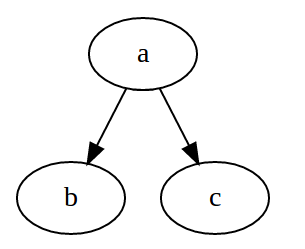
\includegraphics[width=8cm]{bilder/graphVizExample.png}
\caption{Generated graph image from Listing \ref{vizJs}.}
\label{graphVizEx}
\end{figure}
\end{center}
%\section{Motivation}

The ProB standalone application written in Tcl/Tk uses Dotty as library to create visualizations of certain data structures within the ProB application. Unfortunately, these data visualizations are completely missing in both the Java APIs. The intention of this work is to inspect the data visualizations that are available in the Tcl/Tk application and recreate these in the Java 2.0 API. The visualizations should not be hard coded, but should use D3 and the existing webserver structure to create a framework so that similar visualizations can be created in the future using the same principles.

Central to the ProB application is the concept of the state space. The state space is a directed multigraph. The states are saved as vertices in the graph and the operations within the graph are saved as directed edges that transition from one state to another. The main purpose of the ProB software is to verify this state space for inconsistencies. For instance, it is possible to use ProB to find states within the graph that violate the invariant for specification. It is also possible to find states from which there are no further operations possible. This is called a deadlock.

The ProB 2.0 API extracts the information about the existing state space from the ProB CLI and saves it in a programmatic abstraction of the state space. This abstraction saves the information about the different states in a graph data structure using the Java JUNG graph library. The state space object already supports the use of Dijkstra's algorithm to find the shortest trace from the root state to a user defined state. This can be used to find traces that show how an invariant violation or deadlock can be found. What is missing, however, is a visualization of the actual state space itself.

Because the state space is a directed multigraph, this visualization problem is not trivial. It was necessary to find a graph library that would be able to draw a complicated graph. Because the state space varies drastically depending on the machine that is being animated, it was also necessary that the graph library be able to handle graphs of all different shapes and sizes.

A useful feature for the visualization of a state space would also be the ability of the user to manipulate the graph. For instance, the Tcl/Tk version of ProB supports the capability for the user to specify a formula and to merge all states for which the formula evaluates to the same result. Similar functionality was desired for the visualization in the ProB 2.0 API. A useful visualization would also allow the user to specify how the graph should be colored.

Although the visualization of the state space was the focus of this work, there were other sets of data for which a visualization would be useful. The ProB Tcl/Tk version supports a useful visualization of B formulas. The user specified formula is broken down into subformulas and colored so as to specify the value of the formula (e.g. if a given predicate evaluates to true at the specified state, the predicate would be colored green). A similar visualization exists in the ProB 1.3.6 API but not in the ProB 2.0 API.

Another useful visualization that falls into the scope of this work was a visualization of the value of a user defined formula over time. No such visualization exists in any of the ProB applications yet, but it was thought that such a visualization would be relatively simple to generate and useful.
\section{Contribution}

\subsection{Visualization framework}

One of the main issues that had to be dealt with at the beginning of the development process was the issue of how to integrate the visualizations into the ProB 2.0 API. At the time, the software already contained a functioning web server using Java servlets. Since the visualizations are written using Javascript and the d3 Javascript library, they needed to use the same framework. Because the visualizations needed to react to changes that take place during the animation of a model, they needed to be able to communicate with the ProB kernel. In order to accomplish this, a javascript function is invoked when the HTML page is loaded. This javascript sets up an interval so that the servlet that is responsible for the visualization is polled every 300 milliseconds to see if there are any changes. Both the servlet and the javascript function keep track of a counter that functions as a time stamp. This number is sent back and forth. If the javascript function identifies a discrepency between the numbers, it polls the servlet and then updates the visualization.

A problem quickly arose because the servlet is a singleton object. There is only one servlet responsible for all of the visualizations of a particular type. The solution for this was to generate a unique session id for every visualization. Using this id, HTML content for the visualization is generated. When the HTML content is loaded, it calls the correct javascript function which sets up the polling interval and generates the visualization for the calculated data.

Once I implemented a way to integrate the visualization servlets into the ProB 2.0 application, it was still necessary to implement an easy way for the user to interact with the visualizations. One of the main advantages of the D3 visualization framework is the flexibility for the user. Using the D3 selectors, it is possible for the user to select and change the attributes of any of the elements of the visualization. In order to offer this functionality to the users from within the ProB 2.0 application, we decided that we needed to lift the functionality from the javascript level into the existing groovy console in the Java 2.0 API. This was accomplished by creating a \texttt{Selection} object that represents the action that the user wants to carry out in the visualization. Then the \texttt{Selection} object is added to the particular visualization and is applied the next time the visualization is redrawn. The \texttt{Selection} object was written so that its functionality is similar to what the user would actually write using the D3 library.

\begin{verbatim}
\\In the Groovy Console:
\\Define an object to tell the visualization to select the 
\\ circles with ids #croot and #c1 and color them pink
x = viz.selectAll("#croot,#c1").attr("fill","#f36")

\\Add this selection to the visualization with session id "0"
viz.addToSession("0",x)
\end{verbatim}

\subsection{Visualization of the State Space}

During the preliminary experiments for State Space visualization, several different graph libraries were tested out. D3 was chosen because it could process graphs of relatively large size in a way that was eye pleasing for users. Visualization of the state space uses the Spring layout that is available from the D3 library. Unfortunately, when visualizing state spaces with a very large amount of states and inputting them all at the default intitial position, it took rather long for a good visualization to emerge. Therefore, the FRLayout from the JUNG graph library was used as a static rendering engine to calculate the ideal initial positions for the states to be visualized in the graph.

One of the main problems with the web framework that was discovered at the start of the development process was the problem of how different state spaces should be visualized at the same time. The ProB 2.0 API supports the animation of multiple state spaces at any given time. When a state space visualization is created, it is created using the state space that is currently being animated. When the animation is switched, a new state space visualization can be created using the new state space that is being animated. The problem is that a state space visualization is not static. Since the state space that is being visualized changes over time when states are added into the graph, the visualization also needs to adapt and grow correspondingly. The solution to this is to have the instance of the state space visualization poll the state space regularly to get any new states that have been discovered. The problem occured because the servlet responsible for dealing with the state space was static. When the polling occured, the servlet did not know which instance of the state space was supposed to be polled.


(NOT YET IMPLEMENTED)
(ONCE IMPLEMENTED DESCRIBE THE DETAILS OF HOW IT IS IMPLEMENTED)
The visualization of the state space is interactive. The user can grab the nodes within the state space and move them around so that they appear exactly as the user desires. Because it the whole visualization is completely written in d3 and Javascript, it is also possible for the user to interact with the visualization using JQuery to change the appearance of the different objects. 

The user can also input Classical B formulas and thereby filter the graph. This uses the algorithms described in \cite{LeTu05_8}. The formula is applied to the state space and all states are merged for which the formula evaluates to the same result. The result is a smaller state space that can be viewed by the user.

\subsection{Visualization of the Value of a Formula Over Time}

During animation in the ProB 2.0 API, the animation steps that have been taken are saved in a trace. A particular formula can take on different values over the course of a trace. In the implementation of the B state space, a particular state is determined by the different values that a variable takes on. Therefore it is particularly interesting to be able to examine the value of a variable over the course of a trace when dealing with a Classical B or Event B formula. 
Evaluation of a formula for takes place in the ProB prolog core. In the ProB 2.0 API, a feature was implemented that takes the list of all the states that the trace covers and a particular formula and returns the list of the values that the formula takes on in the course of the trace. This feature was used in order to create a line plot of the values that the formula takes on. This works for all formulas that take on either an integer value or a boolean value (IMPLEMENT BOOLEAN VALUE).

\subsection{Visualization of a formula}

The ProB CLI already supported the functionality of expanding a formula into its subformulas and finding its value at a given state. However, this functionality would only return the subformulas that were directly beneath the desired formula. For the visualization, it was desired that a given formula could be completely expanded and evaluated and then sent to the ProB 2.0 API. This would ensure that performance would not become an issue. It is now possible to register a Classical B formula in the core and then access the expanded and evaluated formula.

In order to implement the visualization, the d3 tree layout was used. (ADD DIAGRAM OF VISUALIZATION)

This visualization is interactive. The user can select the nodes to expand or to retract the subformulas. It provides a visualization so that the user can easily interpret the formula. If the formula was evaluated to true for the given formula, the text of the formula is displayed in green. If the formula was evaluated as false, the text is displayed in red. This allows the user to automatically identify the parts of the formula that may have produced the problem. 
%\section{Related Work}

The focus of this work was to apply existing graph algorithms to the problem of visualizing a state space. However, a great deal of work has been done in developing algorithms to simplify the state space so that it can be better visualized. Two algorithms have already been integrated into ProB \cite{LeTu05_8}. One of these, the signature merge algorithm, has already been presented in this work. However, the DFA-Abstraction algorithm presented there has not yet been integrated into the new tool.

Several tools exist specifically for the visualization of directed graphs. Walrus\footnote{http://www.caida.org/tools/visualization/walrus/} and GraphViz\footnote{http://www.graphViz.org}, which has already been introduced in this paper, are two tools that can be used for graph visualization. Some tools which require the visualization of labeled transition systems use the graph visualization features that are provided by these tools. As we have seen, ProB is one of these tools. CSPM\footnote{http://hackage.haskell.org/package/CSPM-cspm} is another tool which supports the generation of DOT files in order to visualize the state space associated with CSP specifications.

However, there are also several tools developed for the specific purpose of visualizing state spaces. Van Ham et al. \cite{Ham02} have considered the problem of visualizing labeled transition systems and developed the LTSView\footnote{http://www.mcrl2.org/release/user\_manual/tools/ltsview.html} tool for visualizing the structure of state spaces. This tool produces a 3D representation of a state space that the user can inspect. In order to simplify the visualizations that are created by LTSView, work has been done to develop a method of converting 3D models of labeled transition systems to 2D \cite{Pretorius2005}. The StateVis tool is the result of this research\footnote{http://www.win.tue.nl/vis1/home/apretori/statevis/}. These tools can help users to get a rough idea of the feel of the whole state space. However, they do not allow for a close inspection of interesting parts of the state space. In order to provide a solution to this problem, Pretorius and van Wijk have proposed a method for interacting with the visualization of state transition graphs \cite{Pretorius2006}. The tools NoodleView\footnote{http://www.comp.leeds.ac.uk/scsajp/applications/noodleview/} and its successor DiaGraphica\footnote{http://www.comp.leeds.ac.uk/scsajp/applications/diagraphica/} attempt to apply this method.

\section{Conclusion}

Over the course of this work, we have shown the feasibility of using D3 to create data visualizations within ProB. It is not only possible to create the desired visualizations, it is also easy to adapt the servlets so that the visualizations are updated to reflect changes made in the course of model animation. The styling for these visualizations can be easily defined by the user. This gives the user a large amount of control over the visualization.

The visualization of the state space was the focus of this work. The visualization that was created is interactive and is automatically updated as soon as states are calculated and cached in the state space. It also can handle relatively large state spaces (TEST THIS OUT TO DETERMINE HOW LARGE!!!!). 

The decision to support GraphViz visualizations in the state space visualization in addition to D3 visualizations took place relatively late in the development process. Using the existing visualization framework, it was possible to implement this feature in a relatively short period of time. This shows that the visualization framework is relatively flexible and can be easily extended.
\section{Future Work}

Future work

%%%%%%%%%%%%%%%%%%%%%%%%%%%%%%%%%%%%%%%%%%%%%%%%%%%%%%%%%%%%%%%%%%%%%%%%
%%%% ENDE TEXTTEIL %%%%%%%%%%%%%%%%%%%%%%%%%%%%%%%%%%%%%%%%%%%%%%%%%%%%%
%%%%%%%%%%%%%%%%%%%%%%%%%%%%%%%%%%%%%%%%%%%%%%%%%%%%%%%%%%%%%%%%%%%%%%%%

\clearpage
\bibliography{references}
\bibliographystyle{alphadin}
%\vspace*{\fill}

\clearpage

\listoffigures

\listoftables

\appendix

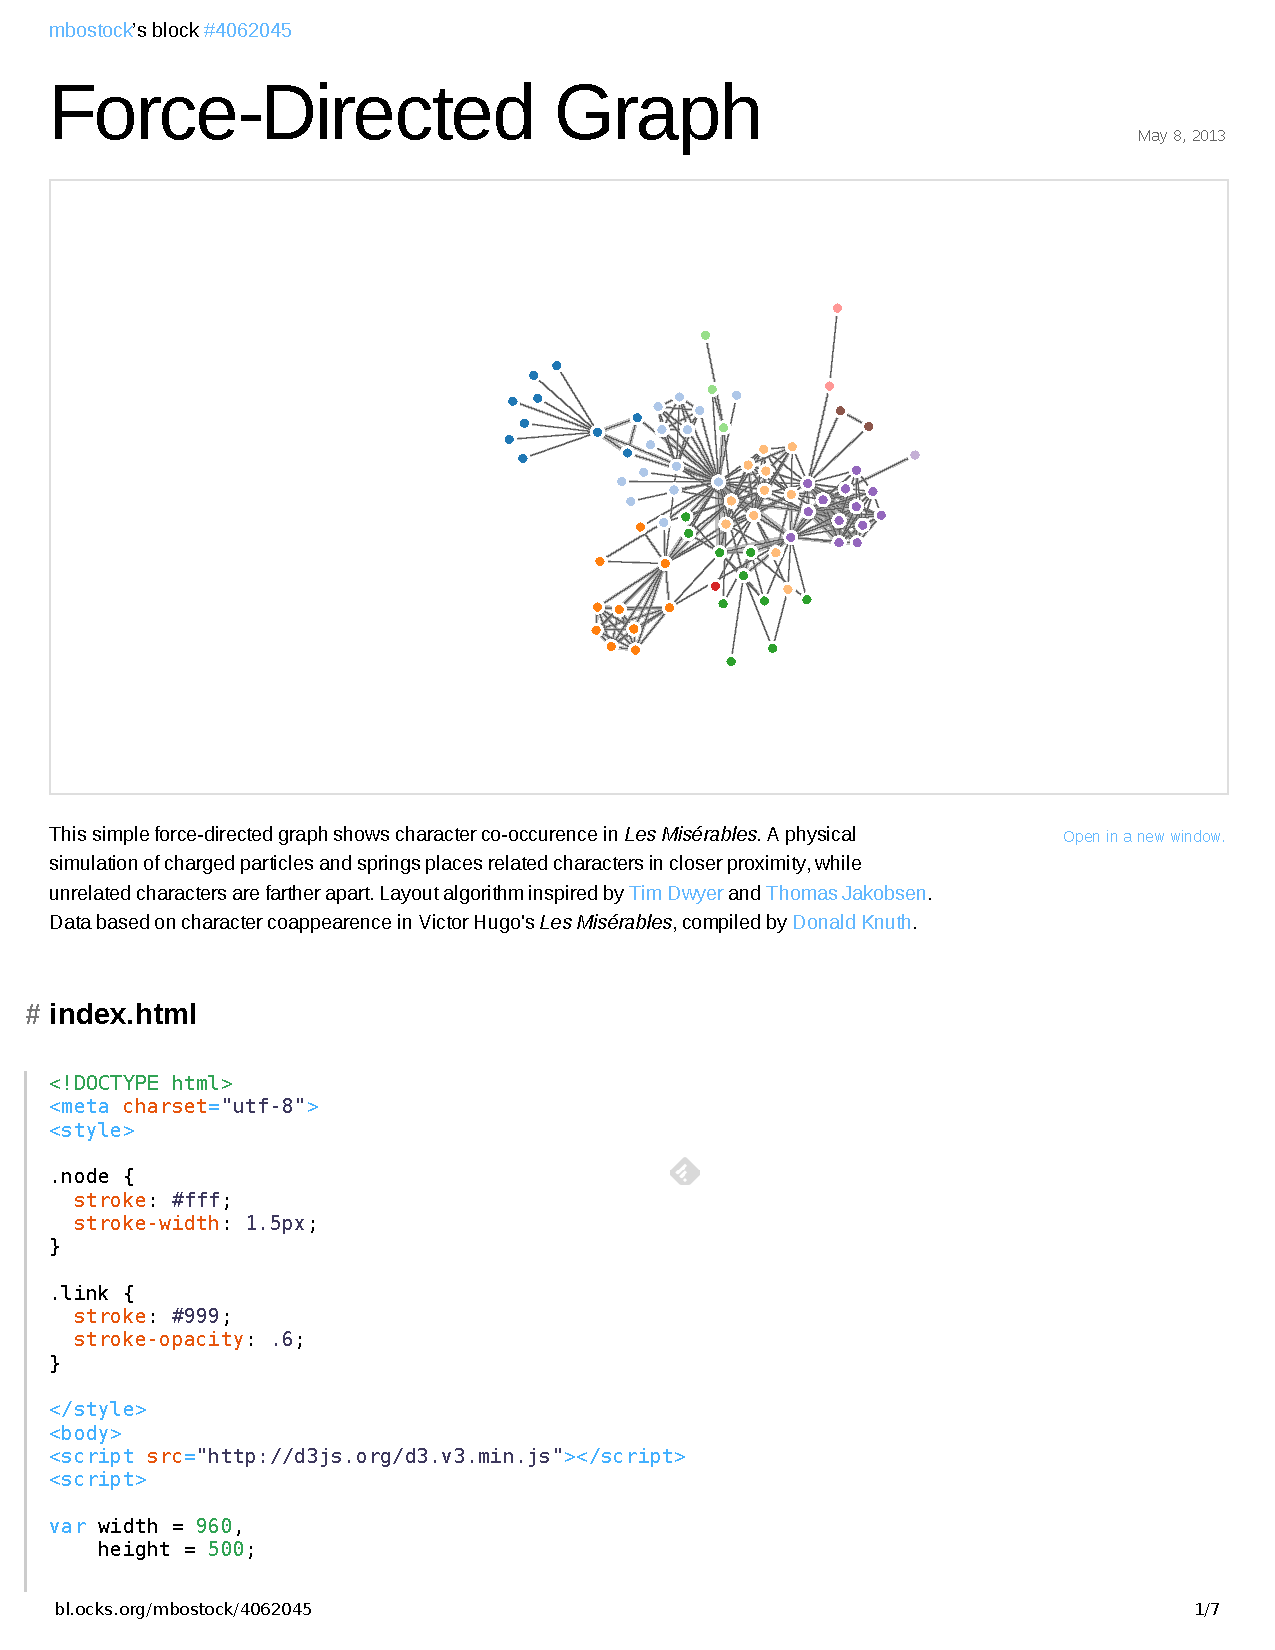
\includepdf[pages=1,pagecommand=\section{Force Directed Graph}\label{appendix:force}, scale=0.75]{appendix/force.pdf}
\includepdf[pages=2-]{appendix/force.pdf}

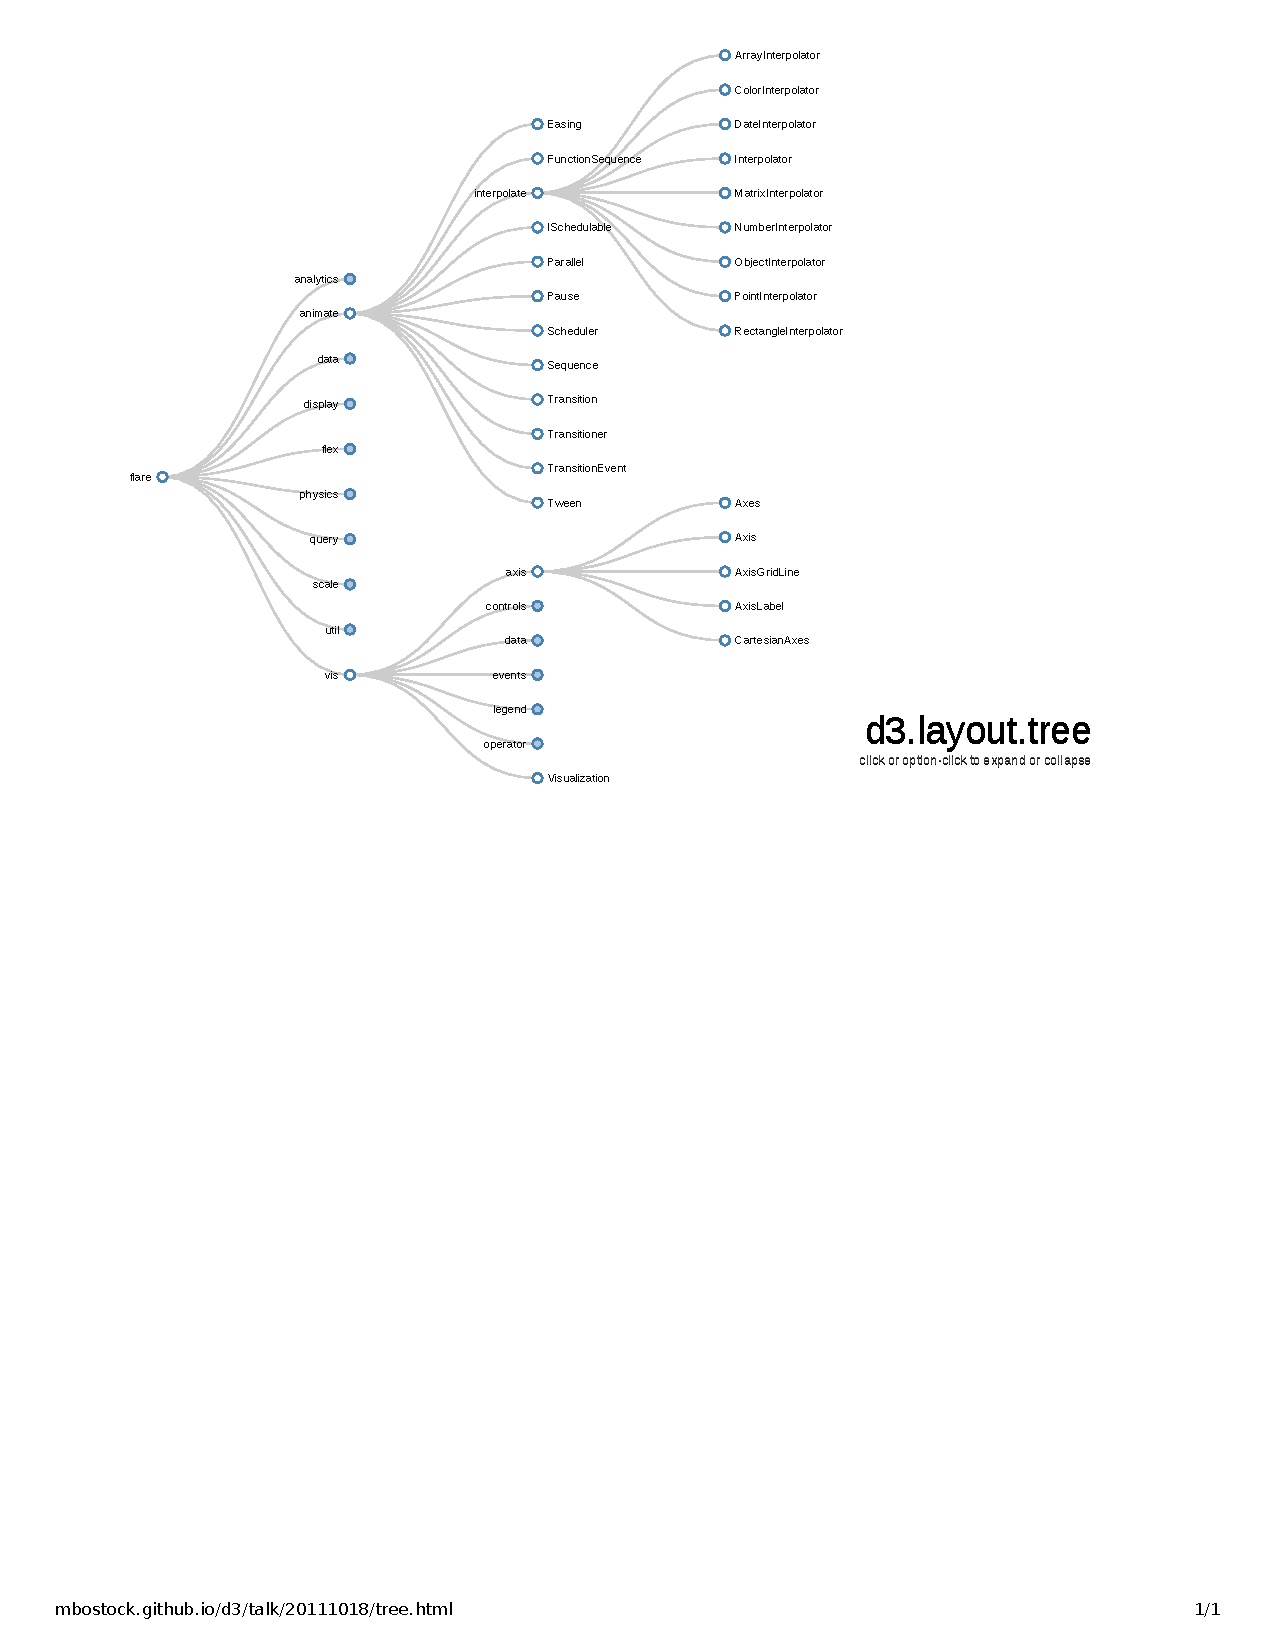
\includepdf[pages=1, pagecommand=\section{Collapsible Tree Layout}\label{appendix:tree}, scale=0.75]{appendix/tree.pdf}
%\pagebreak

%\printindex
\end{document}
